% TeX-command-default: "LaTeX"
\documentclass[12pt,french]{article}
\usepackage[utf8]{inputenc}
\usepackage[T1]{fontenc}
\usepackage{babel}
\usepackage{graphicx}
\usepackage{float}
\usepackage{csquotes}
\usepackage{epigraph}
\usepackage{wrapfig}
\usepackage{rotating}
\usepackage[normalem]{ulem}
\usepackage{amsmath}
\usepackage{textcomp}
\usepackage{amssymb}
\usepackage{capt-of}
\usepackage{lmodern}
\usepackage{hyperref}
\usepackage[margin=1.4in]{geometry}
\usepackage{parskip}
\usepackage{microtype}
\usepackage{gatin} % Personnal styling


\author{SUBLET Gary -- 11506450 \\[.3em] VILLERMET Quentin -- 11507338}
\date{\today}
\title{Intelligence Bio-Inspirée \\[.5em] Travaux Pratiques}

\begin{document}

\gatintitle{Compte-rendu des travaux pratiques sur l'apprentissage profond par renforcement}

\tableofcontents
\newpage

\section{Réplicabilité}
\subsection{Environnement virtuel}

La totalité des expérimentations suivantes ont été réalisées avec Python 3.7, au sein de \textit{notebooks jupyter} et de scripts \textit{.py}.

Afin de favoriser la facilité de reproduction de ces programmes, nous évoluons dans un environnement virtuel, où les modules python peuvent être plus aisément contrôlés. \\
Nos dépendances sont listées dans le fichier \texttt{requirements.txt} à la racine du projet.

Un guide permettant la mise en place de ce \textit{virtualenv} est présent dans le \texttt{Readme.md} du dépôt GitHub.

\section{Deep Q-network sur CartPole}
\subsection{Début}
\subsubsection{Question 1 -- Agent aléatoire CartPole-v1}

Le code de l'agent aléatoire est entièrement contenu dans le fichier \texttt{cartpole.py}, trouvable dans les sources du projet.

Il est presque entièrement basé sur l'exemple des créateurs de \texttt{gym} présent sur le \href{https://github.com/openai/gym}{GitHub} du module.

\subsubsection{Question 2 -- Évaluation des récompenses}

\begin{note}
En plus de l'affichage demandé, nous avons pris l'initiative de créer une visualisation de la récompense cumulée au fil des épisodes dénotant en quelque sorte le \og succès\fg\, de la session d'apprentissage.
\end{note}

Nous avons opté pour un affichage \texttt{matplotlib}, avec \textit{mean-pooling} pour alléger le graphe en cas de grand nombre d'épisodes lorsque nécessaire.

Dans notre premier cas, soit celui d'un agent aléatoire sur l'environnement \textit{CartPole-V1}, le graphe des récompenses cumulées en fonction du nombre d'interactions aboutit forcément à un nuage de points suivant la fonction $f(x) = |x|$.

On constate peu d'\textit{outliers} (qu'on considèrera ici comme ayant $x > 60$), en raison du caractère aléatoire des décisions.

\begin{center}
    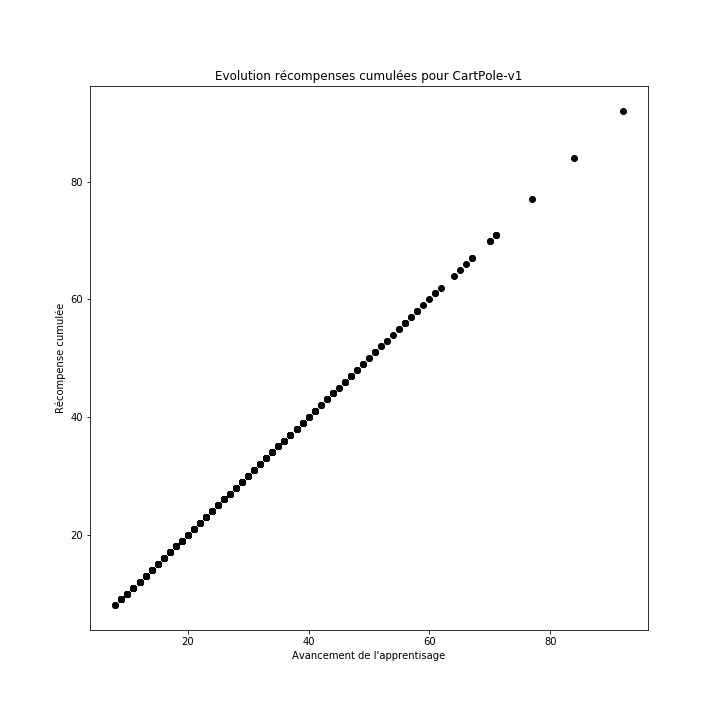
\includegraphics[width=\textwidth]{../src/img/env_CartPole-v1_random_cumu.png}
\end{center}

Ce résultat est sans surprise, puisque toute interaction entraîne une récompense de 1 dans cet environnement.

La deuxième visualisation n'est pour le moment pas très utile non plus, puisque notre agent n'apprend pas et agit de façon aléatoire.

\begin{center}
    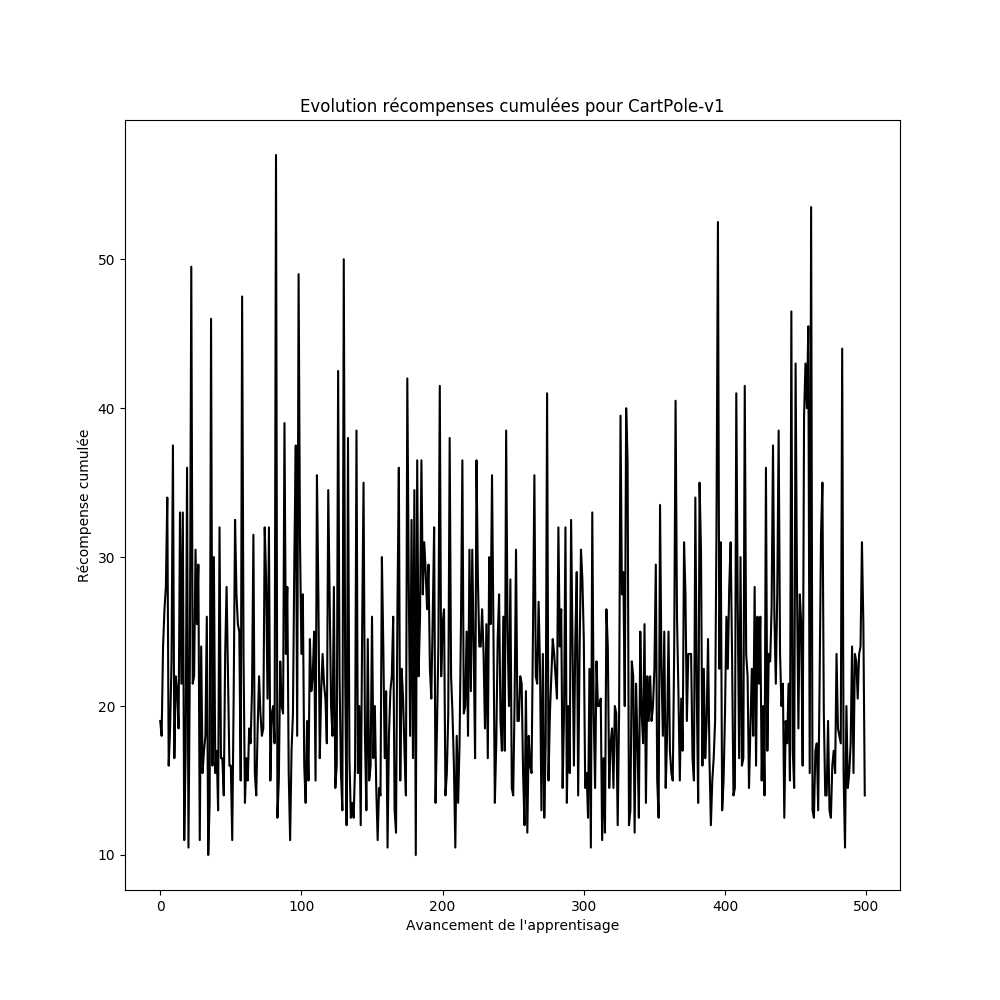
\includegraphics[width=\textwidth]{../src/img/env_CartPole-v1_random.png}
\end{center}

Ces deux affichages prendront leur pertinence plus tard dans le développement, lorsque notre agent commencera à apprendre de son environnement.

Il nous indiqueront respectivement la rapidité d'apprentissage des épisodes individuels, et l'efficacité générale de l'apprentissage en fonction du temps passé (\textit{i.e.} des épisodes).

\newpage
\subsection{Experience replay}

\subsubsection{Question 3 -- Buffer de stockage d'expériences}

Le code du buffer \textit{experience replay} est dans le fichier \texttt{deeprl\_agent.py}, plus particulièrement la fonction \texttt{experience} de la classe \texttt{Agent}.\\
Cette question marque le début du code des notebooks jupyter.

\subsubsection{Question 4 -- Sampling de mini-batch}

À partir de cette question, nous basculons sur un système de notebooks \textit{Jupyter} pour une implémentation plus rapide des tests. \\
La récupération de mini-batch de données du buffer se fait donc dans le fichier \texttt{experience\_replay.ipynb}.

\subsection{Deep Q-learning}

L'implémentation du Q-learning se fait dans la continuation de la partie précédente, donc dans le fichier \texttt{experience\_replay.ipynb}. Sauf indication du contraire, c'est au sein de ce notebook que le reste du TP se déroulera.

\subsubsection{Question 5 -- Réseau de neurones}

Pour notre premier exemple, on construit donc un réseau avec 4 neurones d'entrée et 2 neurones de sortie.

En effet, dans l'environnement \textit{CartPole-v1}, l'observation est de type \texttt{Box(4,)} et le domaine des actions est un \texttt{Discrete(2)} (en l'occurence 0 et 1 pour bouger à gauche et à droite respectivement).

Ces dimensions expliquent la taille de notre réseau.

\subsubsection{Question 6 -- Approximation des Q-valeurs}

Les deux stratégies d'exploitation proposées sont implémentées dans la classe \textit{Agent}, qui est dotée des fonctions \texttt{epsilongreedy(self, ob, epsilon)} et \\\texttt{boltzmann(self, ob, tau)} qui renvoient l'action choisie, qui est soit une action aléatoire d'exploration, soit le choix déterminé par la politique d'après les Q-valeurs prédites par le réseau.

Pour la politique $\epsilon$-greedy, il s'agit de la meilleure action avec une probabilité $(1 - \epsilon)$. Pour Boltzmann, le choix est stochastique mais tend malgré tout à choisir la Q-valeur maximale le plus souvent.

\subsubsection{Question 7 -- Apprentissage}

À ce stade du développement, notre agent utilise désormais toute une panoplie de fonctions ; à chaque fois qu'il doit choisir une action, il fait appel à \texttt{choose\_action(ob, reward, done)}, qui détermine les Q-values avant de déterminer (selon la méthode d'exploration actuelle) l'action choisie.

Après avoir effectué son action, celle-ci est appliquée à l'environnement par le biais de la fonction \texttt{step()}, après quoi on fait appel à l'\textit{experience replay}. Pour ce faire, on utilise la fonction \texttt{experience()} de la classe \textit{Agent.}

À la fin de notre épisode, on utilise \texttt{minibatch()} pour récupérer des expériences passées de l'agent, puis on apprend sur chacune des expérience de cette mini-batch.

\begin{center}
    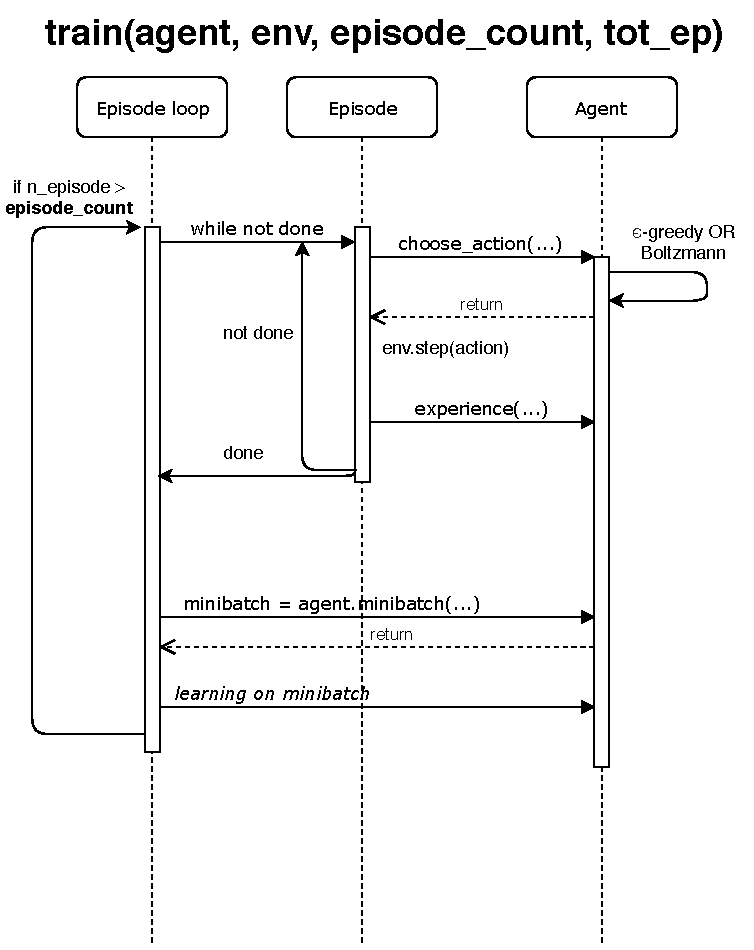
\includegraphics[width=.7\textwidth]{../src/img/Q7.pdf}
\end{center}

Ci-dessus, un diagramme de séquence simplifié de l'entraînement d'un Agent.

\subsubsection{Question 8 -- Target Network}\label{target}

Le \textit{target network} a été implémenté selon la solution \og N-étapes\fg. On calculera donc la Q-valeur ciblée avec ce nouveau réseau, qui sera mis à jour toutes les \textit{N} itérations d'apprentissage. 

Ce \textit{N} se traduira chez nous par l'hyper-paramètre \texttt{target\_sync}, et la fonction \texttt{sync\_target()} d'\textit{Agent} sera appelée en temps voulu.

\subsection{Étude des résultats finaux sur CartPole}

L'apprentissage de notre agent sur l'environnement \textit{CartPole-v1} s'est soldé par un certain succès. Nos premiers pas donnaient parfois un comportement peu optimisé, parfois une politique plus solide, mais après quelques temps et une session d'apprentissage plus longue, on commence à distinguer une réelle progression.

\begin{minipage}{.5\textwidth}
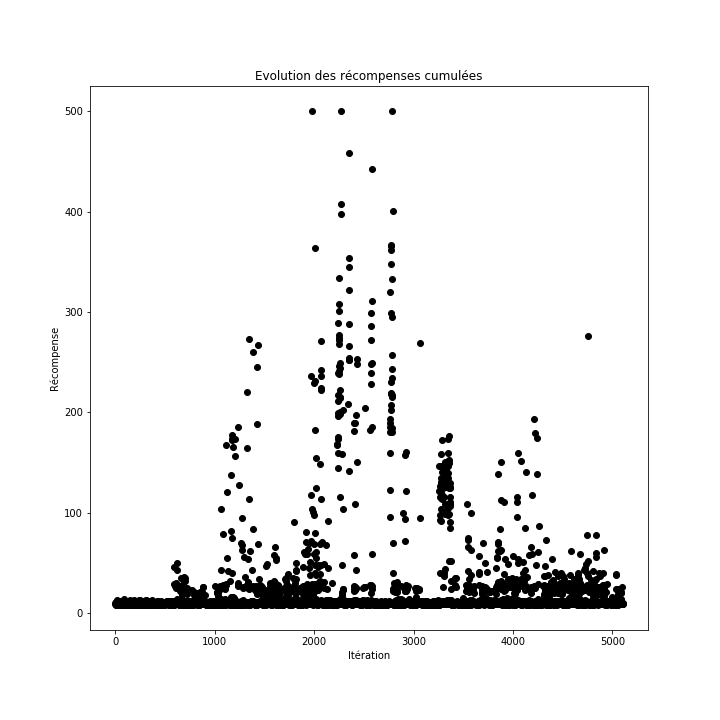
\includegraphics[width=\textwidth]{{../src/img/CartPole-v1/dot_5000_5_e5105_eta0.01}.png}
\end{minipage}
\hfill%
\begin{minipage}{.5\textwidth}
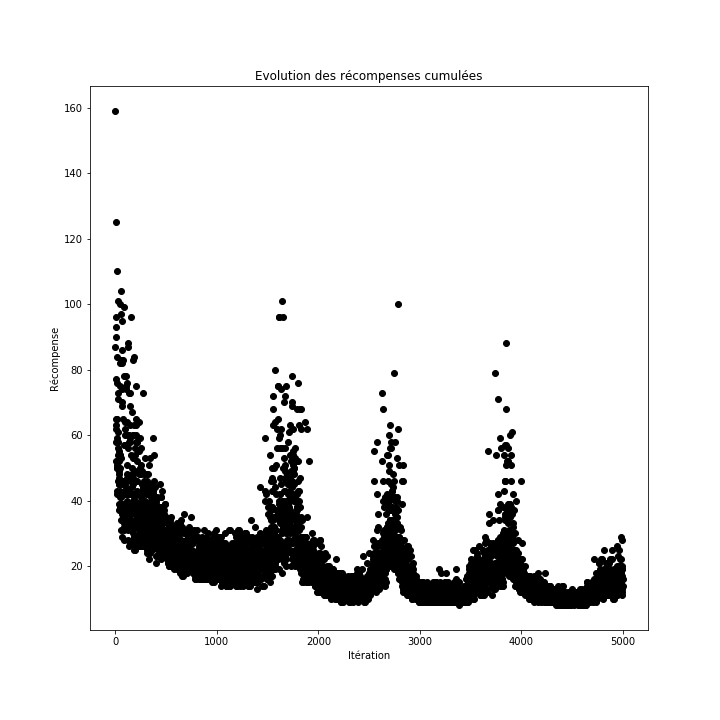
\includegraphics[width=\textwidth]{{../src/img/CartPole-v1/dot_5000_5}.png}
\end{minipage}

Ci-dessus, quelques-un de nos premiers succès représentés graphiquement. Sur seulement 5\,000 itérations, l'agent peut atteindre une récompense de 500 (qui est la récompense maximale de l'environnement) plusieurs fois.

Cependant, on ne constate pas de réelle amélioration sur le long terme de son comportement. L'évolution de sa performance semble au mieux erratique, et on ne pouvait pas se satisfaire d'un tel agent.

Après quelques modifications des hyper-paramètres, toujours sur 5\,000 itérations, on aboutit à de meilleures tendances :

\begin{minipage}{.5\textwidth}
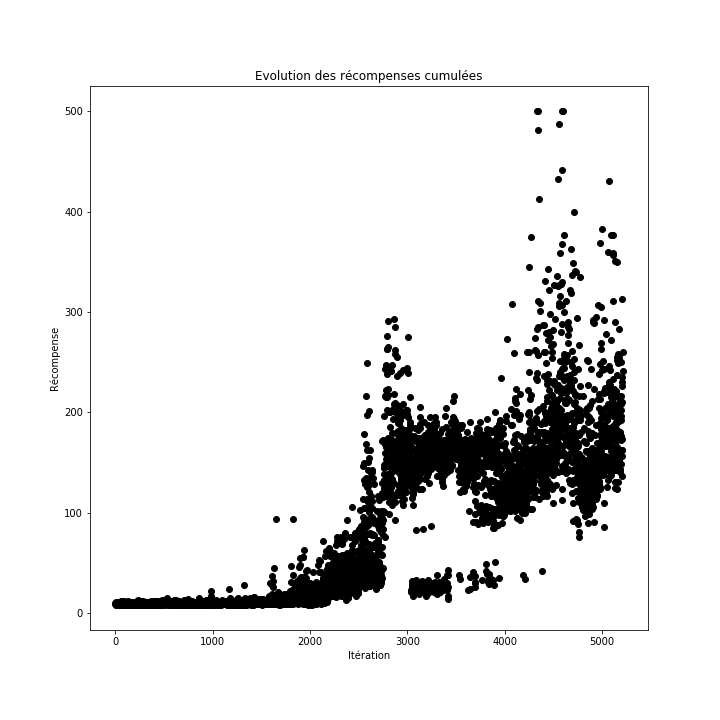
\includegraphics[width=\textwidth]{{../src/img/CartPole-v1/dot_5000_5_e5213_eta0.01}.png}
\end{minipage}
\hfill%
\begin{minipage}{.5\textwidth}
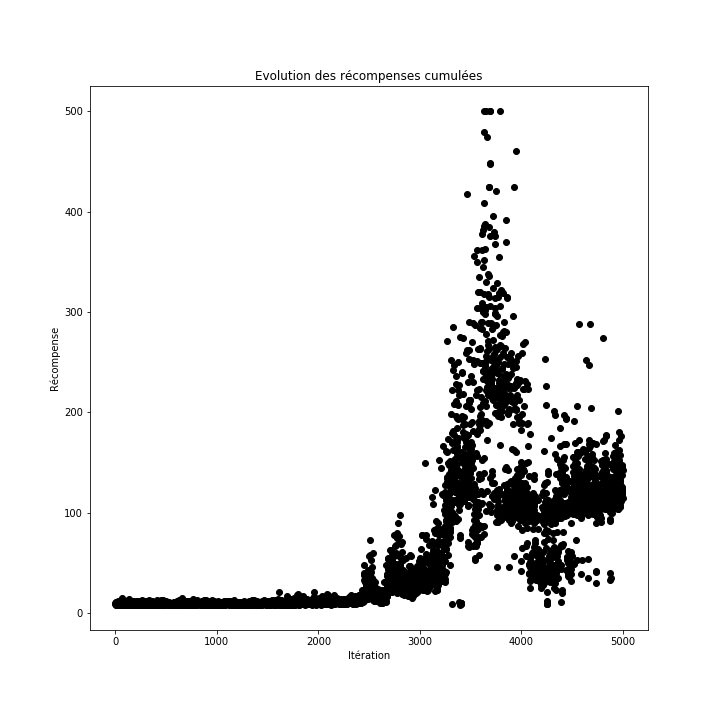
\includegraphics[width=\textwidth]{{../src/img/CartPole-v1/dot_5000_32}.png}
\end{minipage}

Cette fois, l'agent semble mieux \og retenir\fg\, ses bonnes performances passées. On constate déjà une tendance qu'on retrouvera par la suite, celle de \og pallier\fg\, de récompenses cumulées dans le graphique.

En effet, l'agent semble avoir des performances variables, même après un certain apprentissage, mais les récompenses des épisodes tombent le plus souvent dans des fourchettes déterminées.

Il est difficile de déterminer ci ces palliers sont dûs à la nature de l'environnement ou, au contraire, si l'agent lui-même en est la source.\\
Quoi qu'il en soit, nous avons ensuite réalisé de nouvelles sessions d'apprentissage, cette fois en passant à 10\,000 itérations.

Ces nouvelles sessions ont non seulement plus d'itérations, mais sont aussi les premières à implémenter le \textit{target network} de la \hyperref[target]{Question 8}.

Là où les résultats ci-dessus tendent à l'instabilité (en particulier, le deuxième cas présente un apprentissage jusqu'à 500 de récompense suivi d'une retombée assez décevante), l'ajout du deuxième réseau permet de viser une cible stable pendant au moins \texttt{target\_sync} itérations.

Ces deux améliorations nous permettent d'obtenir des comportements plus satisfaisants, qui sont illustrés ci-dessous.

\begin{minipage}{.5\textwidth}
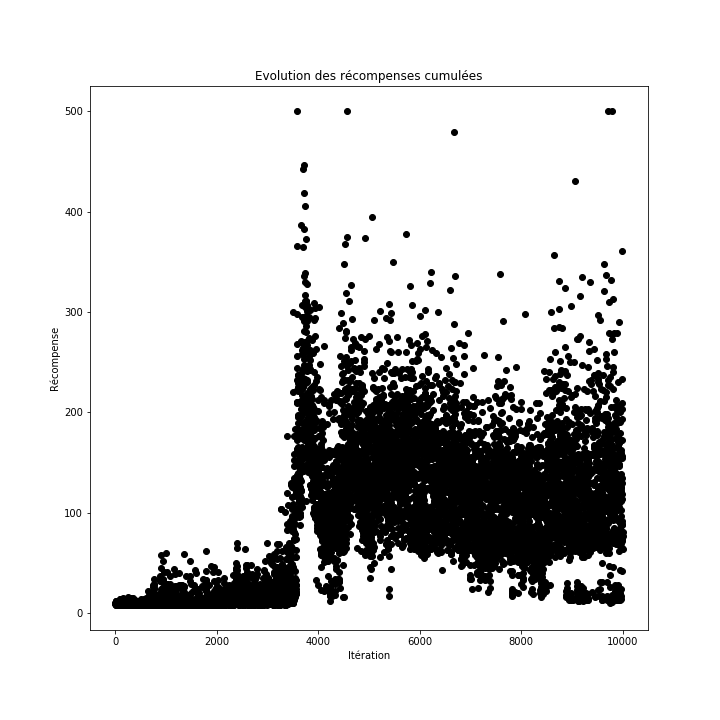
\includegraphics[width=\textwidth]{{../src/img/CartPole-v1/dot_10000_5_e10000_eta0.01_target}.png}
\end{minipage}
\hfill%
\begin{minipage}{.5\textwidth}
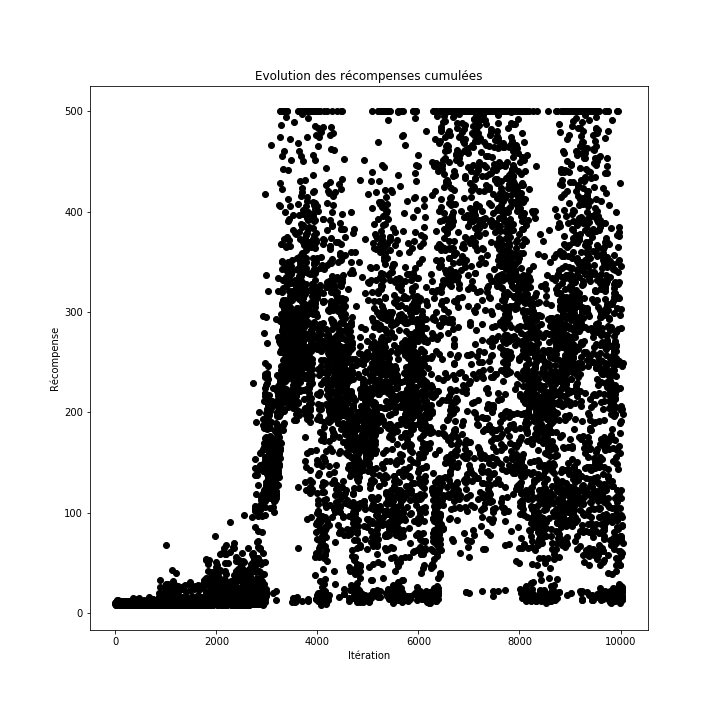
\includegraphics[width=\textwidth]{{../src/img/CartPole-v1/dot_12000_5_e10043_eta0.01_target}.png}
\end{minipage}

L'ensemble de ces résultats ont été obtenus avec $\eta = 0.01$ et un batch\_size de 32. Le phénomène de palliers est ici peu visible, mais se remarque plus facilement sur une session encore plus longue. 

Ci-dessous, notre dernière session, de respectivement 20\,000 et 50\,000 itérations :

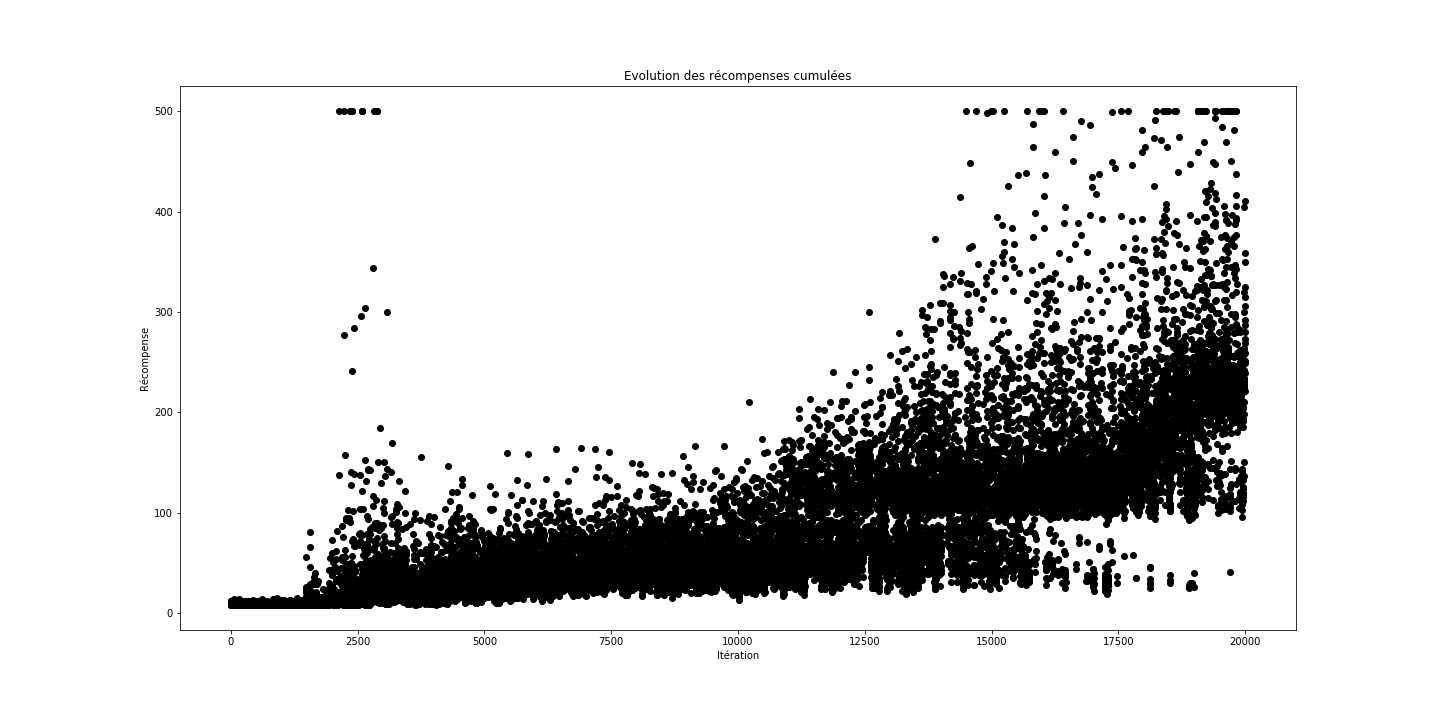
\includegraphics[width=\textwidth]{{../src/img/CartPole-v1/dot_10000_32_e20000_eta0.01_target}.png}

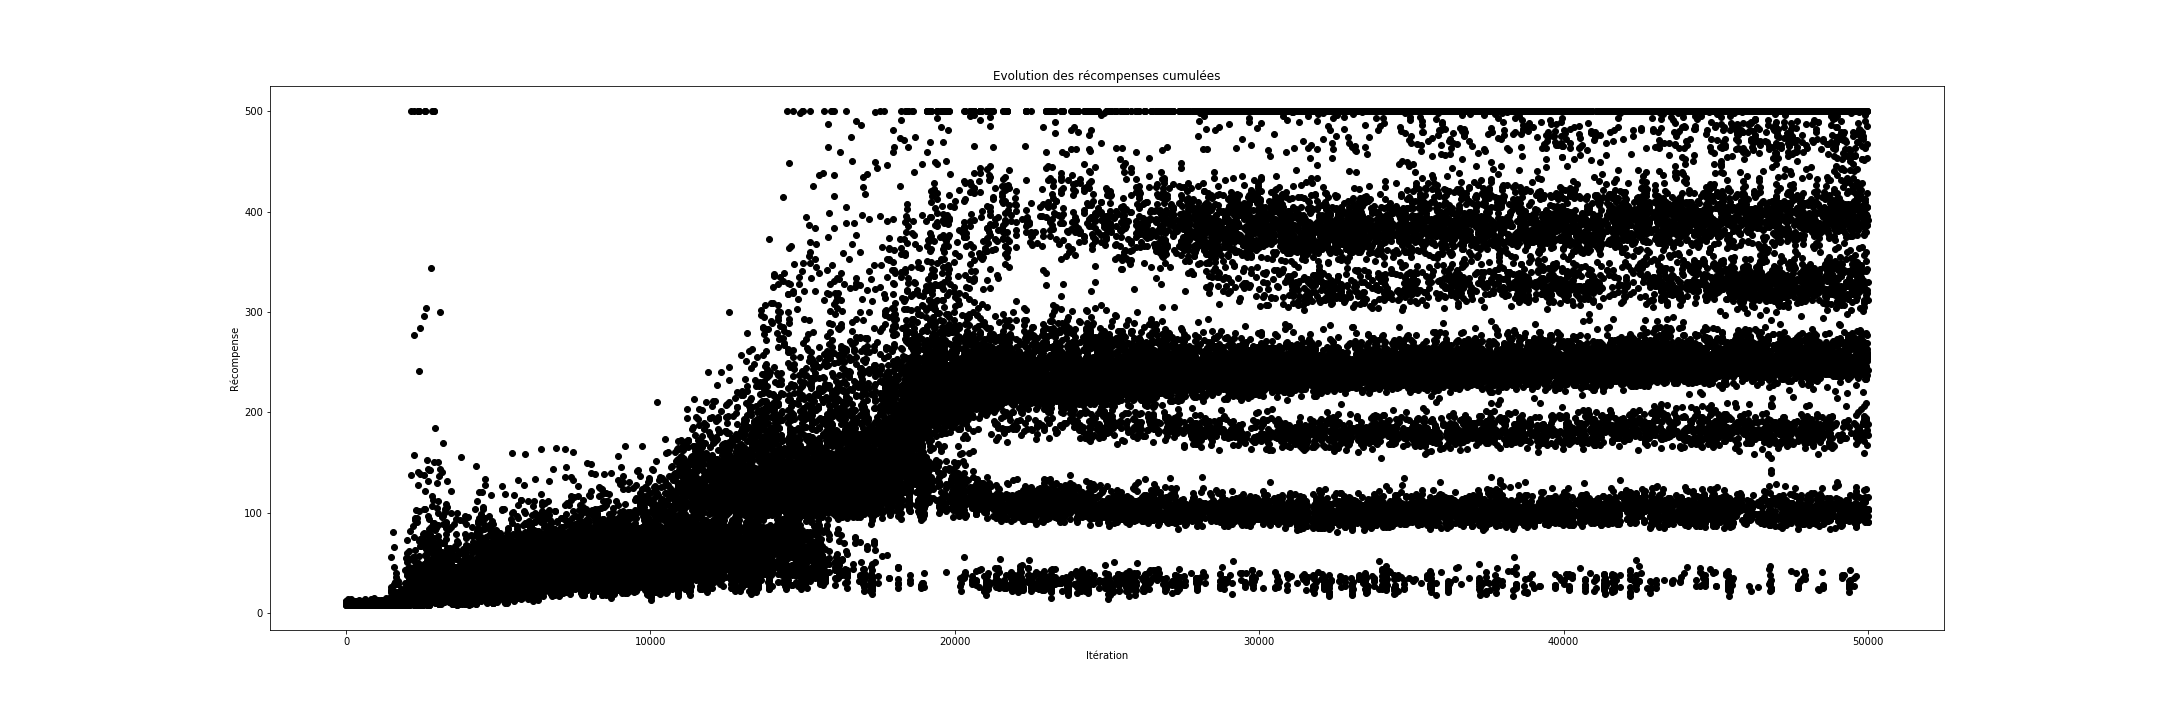
\includegraphics[width=\textwidth]{{../src/img/CartPole-v1/dot_10000_32_e50000_eta0.01_target}.png}

Les deux images représentent la même session, à différents niveaux d'avancement. On constate mieux le phénomène de palliers, et, en particulier, après quelques dizaines de milliers d'itérations, l'agent obtient des résultats plutôt déterminés.

Beaucoup d'épisodes obtiennent un score de 500, et la plupart des autres obtiennent soit zéro (probablement à cause d'une exploration déstabilisant le bâton), soit une récompense contenue dans une fourchette assez restreinte, représentant (d'après notre hypothèse) les politiques de l'agent.

Ces résultats finaux nous paraîssent assez satisfaisants mais, le but ultime de cet agent étant d'évoluer dans l'environnement \textit{Atari Breakout}, il nous faut adapter légèrement notre système pour opérer une transition vers ce nouveau jeu.

\section{Breakout Atari}

Sauf indication du contraire, nous évoluons toujours dans le même notebook, soit \texttt{experience\_replay.ipynb}.

\subsection{Question 1 -- Construction de l'environnement}\label{preproc}

L'ajout de ce nouvel environnement se fait dans un bloc dédié (présent juste sous le bloc d'initialisation de \textit{CartPole-v1}). On utilise le wrapper \textit{AtariPreprocessing} pour obtenir les paramètres décrits dans l'énoncé.

En l'occurence, \texttt{grayscale\_obs=True}, \texttt{frame\_skip=4} et \texttt{screen\_size=84}.

\subsection{Question 2 -- Adaptation du code}

Peu de commentaires sont à faire sur cette adaptation. Les détails du code sont comme toujours présents dans le notebook.

\subsection{Question 3 -- Remplacement par un CNN}\label{cnn}

Afin de simplifier l'implémentation du réseau convolutionnel, nous avons ré-utilisé du code produit lors du TP1 d'intelligence bio-inspiré. Durant celui-ci, nous avions réalisé pour une question bonus un tel réseau. Sa classe dédiée est contenue dans un bloc du notebook.

On peut y retrouver le paramétrage du réseau, qui est le suivant :\\
$\longrightarrow$ Couche 1
\begin{itemize}
    \item outchannel = 32
    \item kernel = 8
    \item stride = 4
\end{itemize}
$\longrightarrow$ Couche 2
\begin{itemize}
    \item outchannel = 64
    \item kernel = 4
    \item stride = 2
\end{itemize}
$\longrightarrow$ Couche 3
\begin{itemize}
    \item outchannel3 = 64
    \item kernel3 = 3
    \item stride1 = 1
\end{itemize}

\subsection{Question 4 -- Optimisation des hyper-paramètres}

La partie \og Methods\fg\, de l'\href{https://web.stanford.edu/class/psych209/Readings/MnihEtAlHassibis15NatureControlDeepRL.pdf?fbclid=IwAR01PCi7tuNhTf-DXgXlPDALdIe_Hj6PGTkcMEGlsFadiQ-FPmtPihvTk-s}{article}, à partir de la page 6, détaille certains éléments et hyper-paramètres, dont le pré-processing (déjà aligné sur l'article depuis la \hyperref[preproc]{Question 1}).

La structure du réseau convolutionnel, détaillée dans la \hyperref[cnn]{Question 3}), est elle aussi déjà calquée sur celle des chercheurs, tout comme la taille des mini-batch de 32 et le taux d'update du \textit{target network} (10\,000).

La taille du buffer d'\textit{experience replay}, elle, doit être adaptée. Nous utilisions jusqu'à présent seulement 10\,000 de taille maximale, comparée aux 1\,000\,000 de l'article.

Ayant ajusté nos paramètres, nous tentons alors de lancer nos sessions d'apprentissage sur ce nouvel environnement.

\subsection{Question 5 -- Vidéos du comportement et réseau}

Malgré les hyper-paramètres optimisés, notre agent semble avoir des difficultés lors de son apprentissage. La plupart de nos premières sessions se terminant avec l'agent collé contre le mur (ce qui s'avère fonctionner dans certains cas particuliers), nous avons cherché une parade à ce comportement peu optimisé.

Nos premières tentatives consistaient à favoriser l'exploration et une vision plus long-terme de l'apprentissage.

En premier lieu, nous avons tenté d'utiliser la stratégie $\epsilon$-greedy avec un $\epsilon$ non pas fixé à 0.05 mais décroissant en partant de 1, comme l'a été fait dans l'article référencé précédemment.\\
Ainsi, l'agent est forcé à une exploration aléatoire durant ses premiers pas d'apprentissage. Cette stratégie n'a malheureusement pas porté ses fruits.

Toutes nos tentatives d'apprentissage se sont soldées par un échec, l'agent ayant atteint un grand maximum de 13 points. Il semble s'être coincé dans le premier comportement augmentant légèrement sa récompense, en se collant systématiquement au côté de l'espace de jeu.

\begin{center}
    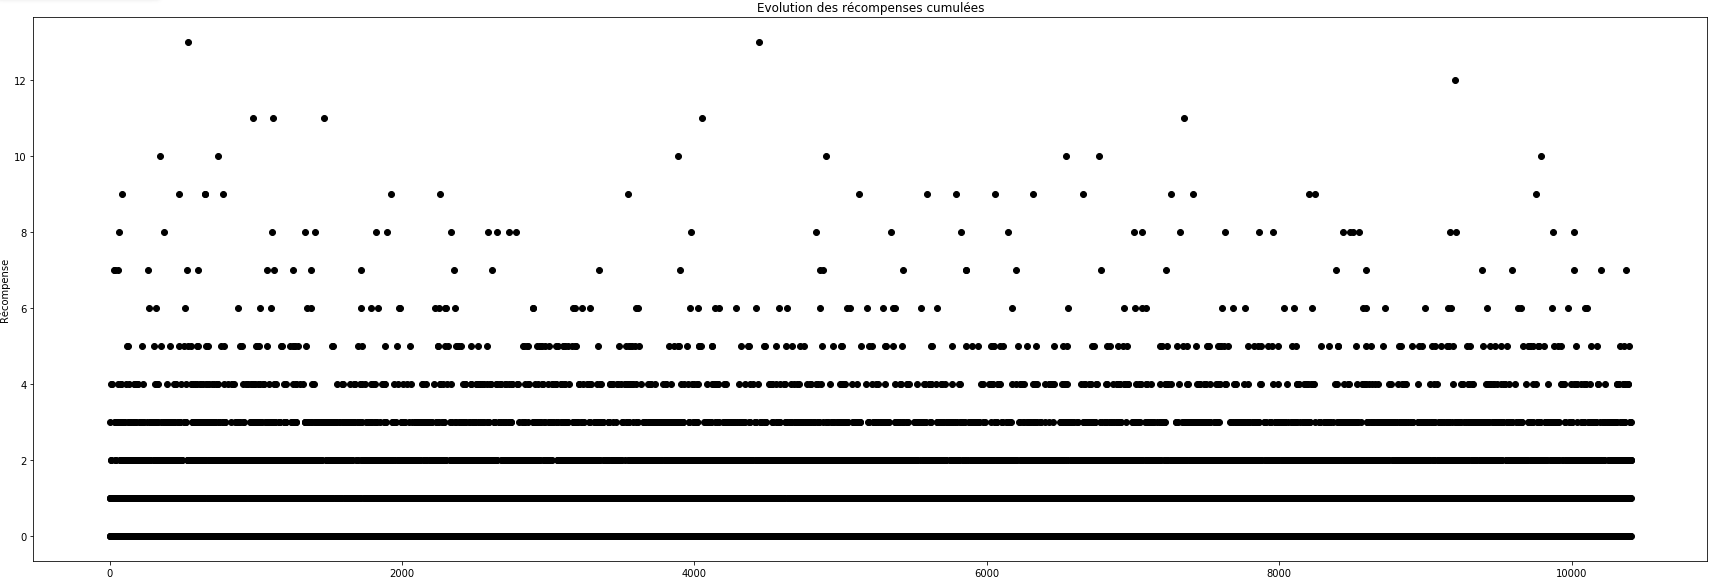
\includegraphics[width=\textwidth]{../src/img/atari_fail.png}
\end{center}

Malgré tout, nous avons enregistré comme demandé des vidéos du comportement de l'agent dans le dossier \texttt{vid}, et nos modèles de réseaux de neurones dans le dossier \texttt{model}.

Ces performances peu satisfaisantes auraient potentiellement pu être améliorées avec plus de temps, ou tout du moins plus de temps d'apprentissage.

\end{document}
